\section{Introduction}

\subsection{Présentation du problème}

Dans le cadre de ce problème, on dispose de $n$ robots endormis et un robot éveillé sur un plan. Le robot éveillé va chercher à réveiller les autres robots avec l'aide de ceux qu'il aura pu réveiller sur sa route.

\begin{figure}[h!]
  \centering
  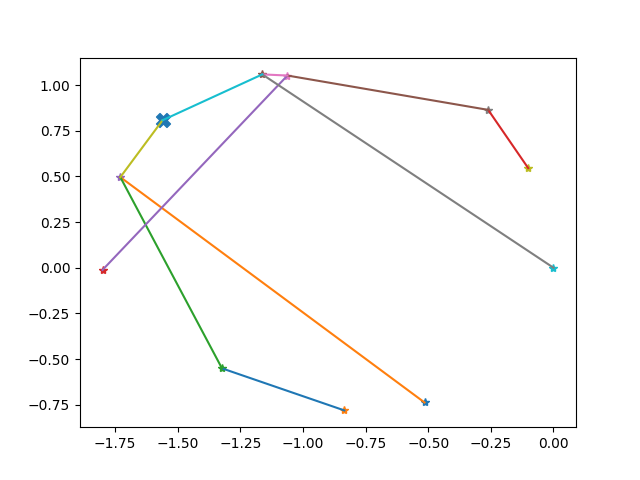
\includegraphics[scale=0.4]{opt_non_plan}
  \caption{Exemple de réveil}
  \label{fig:opt_non_plan}
\end{figure}

Sur cette figure, on commence par deux robots éveillés au niveau de la croix qui vont chacun réveiller un robot qui à leurs tours vont aller en réveiller d'autres selon les segments de couleurs de la figure.

Dans le cas général, trouver le chemin réveillant tous les robots endormis le plus vite possible est un problème NP-dur. Le meilleur algorithme existant, traçant le chemin des robots quelque soit l'emplacement des robots consiste en une programmation dynamique avec une complexité de $\frac{3^n}{\sqrt{n}}$ où $n$ est le nombre de robots endormis.

On peut aussi s'intéresser à la pire configuration possible pour un nombre de robots endormis donné afin de majorer le temps de réveil. On appelle la borne du temps de réveil pour $n$ robots $\alpha_n$. Cette borne est cependant très compliquée à calculer. On connaît la valeur pour $n = 1$,$2$,$3$ et $4$ mais après, les valeurs sont inconnues.

\subsection{Formalisation}

\subsubsection{problème du réveil des robots}

Dans ce rapport, nous travaillerons sur le plan muni de la distance
euclidienne (voir \cite{} pour d'autres métriques). Le robot réveillé débute en
$(0,0)$ et une instance du problème consiste en $n$ points représentant chacun
un robot endormi. Quitte a renormaliser, on supposera que les robots sont
disposés dans le disque de rayon 1 et de centre $(0,0)$. On représente une
solution au problème du réveil des robots par un arbre binaire couvrant tous les
sommets, enraciné en $(0, 0)$. En effet, en chaque sommet un robot entre et
réveille un autre robot: on dispose alors de deux robots à déplacer si on le
souhaite, formant ainsi un arbre binaire dont la racine est le premier robot
éveillé.

En pondérant les arêtes de notre arbre par la longueur de l'arête, on définit la
profondeur de l'arbre comme étant le maximum de la somme des poids des arêtes depuis la racine jusqu'à une des feuilles de l'arbre. Le temps de réveil d'un arbre $T$ est exactement la profondeur de celui-ci, on le notera
$\tr(T)$. L'objectif étant de réveiller les robots le plus rapidement possible,
le temps de réveil optimal est définit comme
$$\min_{\substack{T \text{ arbre binaire couvrant}\\ \text{enraciné en $(0,0)$}}} \tr(T, x_1, \dots,
  x_n).$$

À nombre de robots $n$ fixé, le ``pire'' cas est donc
  $$\alpha_n := \max_{x_1, \dots, x_n \in \mathbb{R}^2} \min_T \tr(T, x_1, \dots,
x_n)$$

Il est assez facile de prouver que  $\alpha_1 = 1$ et $\alpha_2 = \alpha_3 = 3$.
Pour $n=4$, on peut prouver (\cite{}) que $\alpha_4 = 1 + 2\sqrt{2}$.
Gavoille, (lister les autres) ont prouvé dans \cite{} que $\alpha_n \leq 3 +
\frac{8\pi}{\sqrt{n}}$. Il est possible de faire mieux en pratique mais la borne
ferait intervenir une constante plus compliquée que $8\pi$.

Dans la suite, nous utiliserons régulièrement le résultat suivant dû à Gavoille
( et...) :
\begin{theorem}[\cite{}]\label{coneworst}
  Il faut au plus $r(1 + \chord(\theta))$ pour réveiller tous les robots dans un
  cône de rayon $r$ et d'angle $\theta$, à partir d'un robot éveillé
  initialement placé au centre du cône.
\end{theorem}